\documentclass[10pt, conference, compsocconf]{IEEEtran}

% packages
\usepackage{algorithm}
\usepackage{algorithmic}
\usepackage{amsfonts} % for R symbol (the set of real numbers)
\usepackage{color}
\usepackage[pdftex]{graphicx}
\usepackage{graphicx}
\usepackage[bookmarks=false]{hyperref}
\hypersetup{colorlinks=true,linkcolor=black,citecolor=black,filecolor=black,urlcolor=blue}
\usepackage{mathtools}
\usepackage{multirow}
\usepackage{stmaryrd} % for llbracket and rrbracket
\usepackage{subcaption}
\DeclarePairedDelimiter{\ceil}{\lceil}{\rceil}
\DeclarePairedDelimiter{\floor}{\lfloor}{\rfloor}

% new commands
\newcommand{\todo}[1]{\marginpar{\parbox{18mm}{\flushleft\tiny\color{red}\textbf{TODO}:
      #1}}}

\newcommand{\note}[1]{
  \color{blue}\emph{[Note: #1]}
  \color{black}
}

\begin{document}

\title{Predicting computational reproducibility of scientific pipelines using collaborative filtering}

\author{Soudabeh Barghi, Lalet Scaria, Tristan Glatard\\
  Department of Computer Science and Software Engineering\\ Concordia University, Montreal, Quebec, Canada\\
  {first.last}@concordia.ca\\
  $^*$ These authors have contributed equally
}

\maketitle

\begin{abstract}
\end{abstract}


\section{Introduction}

Computational reproducibility, the property through which
computational results can be recomputed over time and
space~\cite{stodden}, has become a critical component of scientific
methodology with the rise of the reproducibility crisis in several
domains~\cite{xxx}. Among the factors hampering computational
reproducibility, infrastructural characteristics such as the operating
system play an important role. In neurosciences, our primary field of
interest, several studies have shown the effect of the operating
system on computational results. However, conducting such
reproducibility studies at scale is cumbersome due to the execution
time of data analysis pipelines, which easily exceeds a few hours.

In this paper we investigate approximate methods to predict the
reproducibility of a computational analysis from the first files that
it produces. Our main intuition is that reproducibility errors are
caused by a reduced number of factors that originate in the analysis
pipeline and input data. 

% Computational reproducibility is an issue, for instance among
% different operating systems (refer to Glatard FINF 2015,
% Gronenschild 2012).

% Scientific data analysis pipeline executions are long (give examples
% from neuroimaging).

% Refer to Germain et al 2008.

% Define subjects, pipelines.

% Problem: predict the reproducibility of pipeline files from other
% subjects and the first files produced by a pipeline. Restrict the
% study to binary classification.




\section{Method}

what is specific to our problem compared to regular collaborative filtering:
%+ subjects are equivalent to users. Not all subjects have the same input data. Anatomical variability, acquisition variability (e.g., 1 subject may have multiple T1s).
%+ files are produced in a specific order (movies aren't),
% which add constraints on the training set (cannot sample late files and not early ones).
%+ utility matrix is not sparse: we can potentially populate it completely. Which means that we can decide precisely which samples we need (active sampling). Therefore we can take the first row and first column to avoid cold start issues.

\subsection{Collaborative filtering using ALS}

% Summarize Koren, Bell and Volinsky: https://dl.acm.org/citation.cfm?id=1608614

% Explain that you have binary classes (rounding)

% Biases

\subsection{Sampling the Training Set}

We investigated the following sampling techniques for the training set. 

% Explain all sampling techniques (maybe rename 4, 5, and 6)
% 1. random unreal (baseline)
\paragraph{Random unreal}
The training set is sampled randomly with no restriction, that is,
regardless of their generation time.  This method will be used as a
baseline for comparison with other methods, although it is not
realistic.~\ref{fig:Random-Unreal-Sample-Training-set}
\begin{figure}
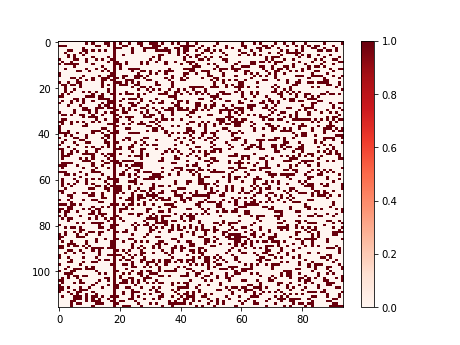
\includegraphics[width=\columnwidth]{figures/5vs7_random-unreal_03_training}
  \caption{Sample training set of random Unreal method with 0.3 training ratio in condition pair of CentOS~5 vs CentOS~7}
  \label{fig:Random-Unreal-Sample-Training-set}
\end{figure}

Note: In the following provided methods in order to overcome the cold start problem and ensure that there is 
at least one sample from each subject and also from each file in the training set, the first generated file of each 
subjects and the whole files of the first random subject are sampled into 
the training set by default. 

% 2. columns
\paragraph{Complete columns}
The training set is sampled by randomly selecting complete columns in
the matrix, that is, complete subject executions. The last selected
column might be incomplete to meet the exact training ratio. This
method is realistic: it corresponds to a situation where the
collaborative filtering method will predict the reproducibility in the
remaining subjects from the subjects in the training set. ~\ref{fig:Columns-Sample-Training-set}
\begin{figure}
  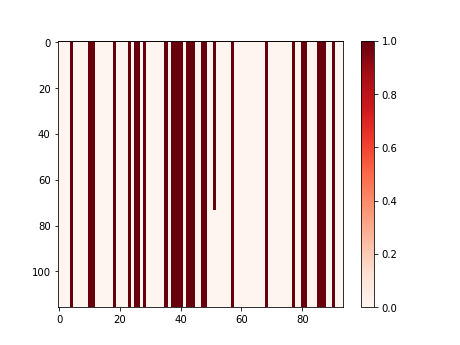
\includegraphics[width=\columnwidth]{figures/5vs7_columns_03_training}
  \caption{Sample training set of Columns method with 0.3 training ratio in condition pair of CentOS~5 vs CentOS~7}
  \label{fig:Columns-Sample-Training-set}
\end{figure}
% 3. rows
\paragraph{Complete rows} The training set is sampled by selecting complete 
rows in the matrix, that is, the first files in
every execution. The last selected row might be incomplete to meet the
exact training ratio. This method is realistic: it corresponds to a
situation where the processing of all the subjects is launched and
interrupted before the execution is complete. The collaborative 
filtering method will then predict the reproducibility of the
remaining files.~\ref{fig:Rows-Sample-Training-set}
\begin{figure}
  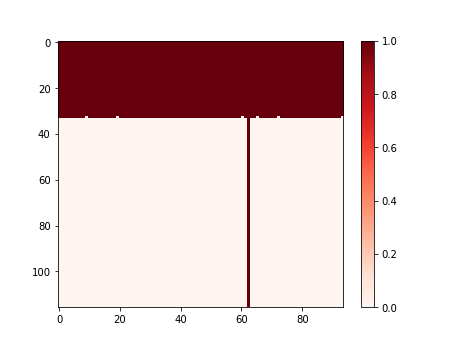
\includegraphics[width=\columnwidth]{figures/5vs7_rows_03_training}
  \caption{Sample training set of Rows method with 0.3 training ratio in condition pair of CentOS~5 vs CentOS~7}
  \label{fig:Rows-Sample-Training-set}
\end{figure}

% 4. random real
\paragraph{Random real (Uniform-S)}
\todo{Explain this better}The training set sampling in this method is quite simillar to complete rows method.
The key difference lies in the way that the next subject is selected randomly. In this respect, subjects' files
are selected by coming their turn which is defined according to their generation time in the pipeline.~\ref{fig:Uniform-S-Sample-Training-set}
\begin{figure}
 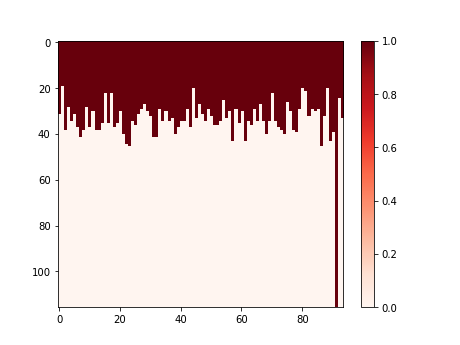
\includegraphics[width=\columnwidth]{figures/5vs7_random-real_03_training}
  \caption{Sample training set of random Real method with 0.3 training ratio in condition pair of CentOS~5 vs CentOS~7}
  \label{fig:Uniform-S-Sample-Training-set}
\end{figure}

% 5. random diagonal
\paragraph{Random diagonal (Uniform-SF)}
The training set suffers from lacking the files which are almost generated towareds the end of pipeline.
In this regard, the number of sampling files' of each random subject is calculated according to a 
uniform distribution which illustrates a diagonal pattern of sampled files from the utility matrix.
\todo{random difference tagert ratio and the efficiant one could be more than 0.01 and less than 0.1}
\begin{comment}
random difference tagert ratio and the efficiant one could be more than 0.01 and less than 0.1
\begin{comment}
\end{comment}

% 6. random triangular
\paragraph{Random triangular}
The training set is sampled by randomly selecting subjects in the matrix.
The number of their files to be sampled in training set is calculated according to triangular distribution.
This ununiform distribution targeting to sample files which are generated almost the end of pipeline by 
meeting the closest training ratio to the requested one by user.
Two approches are tried to apply this method.  

\subparagraph{Largest-a}	
In this approach there is a concern to eliminate the possibility of having less 
than the two first generated files of any subjects in the sampled training set. 
The possibility of missing some subjects in training set can happen to some of them due to 
random selection of subjects or even meeting the determined training ratio before 
having the chance of being selected.

\subparagraph{smallest-a}
In this approach of utilizing triangular distribution,despite of Largest-a approch, there is a possibility 
that some subjects be reperesented in the training set just by their first generated file and no more files.

% For every method, show a training matrix to illustrate for a given ratio. 

\todo{Find better names: consistent with either the graphical patter or the distribution.}
\todo{Add a summary figure of the sampling methods.}

\section{Dataset}

We acquired data about the computational reproducibility of analysis
pipelines of the Human Connectome Project~\cite{general-hcp}. We
processed a set S of 94 subjects randomly selected in the S500 HCP
release~\todo{URL} in three execution conditions with different
versions of the CentOS operating system (5.?, 6.? and 7.?), using the
PreFreesurfer, Freesurfer, PostFreesurfer and fMRIVolume pipelines
described in~\cite{hcp-pipelines} and available at \todo{URL}. For
each pipeline, we identified the set F of files produced for all
subjects in all conditions. For each condition pair and each pipeline,
we computed a binary difference matrix D of size $|F|\times|S|$, where $D_{i,j}$ is true
if file $i$ of subject $j$ was different in each condition. Rows of
$M$ are ordered by ascending file modification time in the pipeline.

Figure~\ref{fig:pre-freesurfer-5-7} shows the difference matrix
obtained for the PreFreesurfer pipeline\todo{Remove title from figure,
  remove color scale, add axes labels.}. The computational
reproducibility of the PreFreesurfer pipeline varies across subjects,
which motivates our study. Nevertheless, some files behave
consistently across all subjects, leading to complete black or white
lines. The ratio of positive elements in this matrix is
\todo{x}\%. Similar matrices were obtained with this pipeline for
CentOS~6 vs CentOS~7 and for CentOS~5 vs CentOS~6, see
Figures~\ref{fig:pre-freesurfer-5-6} and~\ref{fig:pre-freesurfer-5-7}.

\begin{figure}
  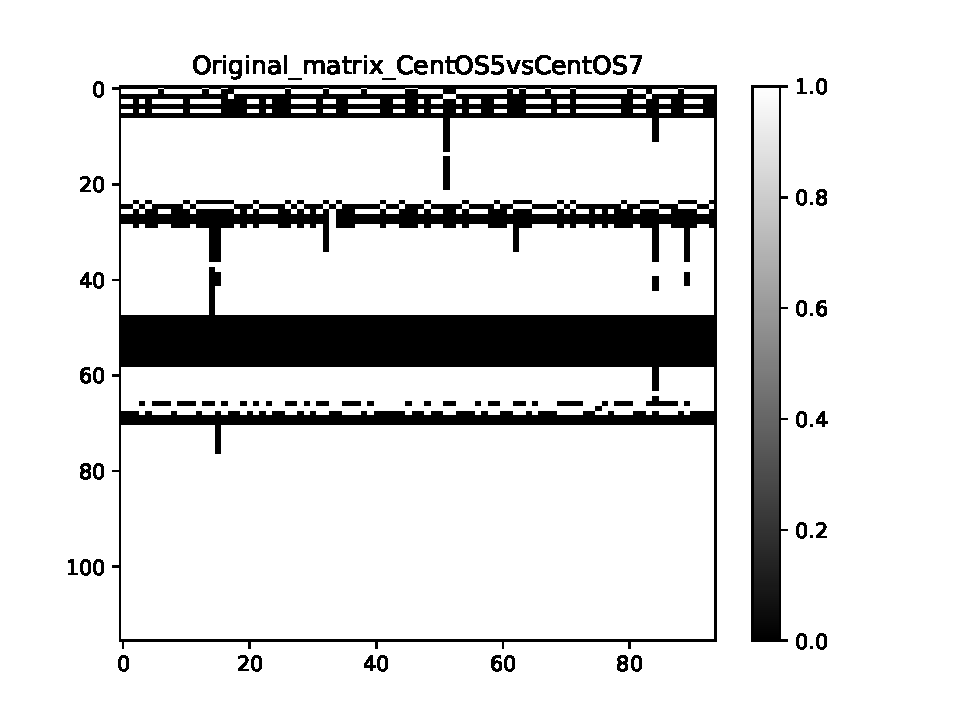
\includegraphics[width=\columnwidth]{figures/original_matrix_CentOS5vsCentOS7.pdf}
  \caption{Difference matrix, PreFreesurfer pipeline, CentOS~5 vs CentOS~7.}
  \label{fig:pre-freesurfer-5-7}
\end{figure}

% Describe your dataset: pipeline(s) used, input data, operating systems (CentOS5, 6, 7), matrix.

% 1. Prefreesurfer (what you have)
% 2. Freesurfer, with the same subjects as in Prefreesurfer.
% 3. PostFreesurfer
% 4. fmriVolume

\section{Results}
The experimental results have been obtained from four different approaches:
1. Straightforward results by applying ALS technique
2. Results achieved through employing Bias as well as ALS technique
3. Results just got through Bias 
4. Results stemmed from ommiting the impact of predicted value for canstant files 
In all above approaches, dummy classifier which makes predictions using simple rules\cite{URL}has been used to indicate that how much predicted value would tend to be anticipate as the dominent value of the utility matrix. This classifier is considered as an accuracy evaluator since the binary utility matrix is consist of \{1,0\} which respectively represent whether a difference has been observed between the same files in two different conditions (by comapring their checksums) or not.
With the knowledge of the fact that random-unreal method is not applicable to our case study we used its results as the comparision between the unrealistic method and realistics ones. In this regard, the aformentioned approaches are propossed and tried to lessen the gaps between the best results from random-unreal and the applied one.
\subsection{Straightforward results by applying ALS technique}
Results show that in all condition pairs Complete Column method has almost a constant accuracy even if the training ratio increased and it is almost two times less than dummy accuracy in more differentiated condition pairs (CentOS5 vs CentOS7 and CentOS6 vs CentOS7). But in the best case which it means in similar conditions the Complete column accuracy is as much accurate as the Dummy accuracy is, \num{0.65} percent.
In general the accuracy pattern of the two complete Rows and Uniform-s methods show similar decline and grow behavior over the training ratio axis however it can be subject to considerable fluctuations in differentiated condition pairs. Dispite of their seemingly irrational behaviour, they always perform a better accuracy for the training size with less than \num{0.3} in comparison to other methods. This better performance (around 75 percent)is almost three times higher than other methods in condition pairs with more differences but just 20 percent better when the conditions are more similar to each other (CentOS5 vs CentOS6) with accuracy of \num{90\%}.
All the other random methods, Uniform-SF and both Triangular approaches are performing a continues groth. Although some considerable variation for both triangular approches have been observed (CentOS5 vs CentOS6) their constant rise leads us to the next phase of experiments which was adding up bias into the current ALS technique. 





% Present your results: accuracy, ROC curves, transparency matrix, factors. 

% Try with different numbers of factors. 

\section{Discussion}

% Not all subjects behave the same, which motivates the Big Data approach. 

% Which sampling method is best

% Interpreting the factors? Factors reflect the pipeline definition. 

% How can this be used in practice

% What are the limitations

\section{Conclusion}

% Summary of the results and discussion. The take-home message.

\section*{Acknowledgment}

\bibliographystyle{IEEEtran}
\bibliography{IEEEabrv,biblio.bib}


\end{document}
